\documentclass[a4paper]{ltjsarticle}
\usepackage{graphicx}
\usepackage{enumitem}
\usepackage{siunitx}
\usepackage{multirow}
\usepackage{cprotect}

\setlist[enumerate,1]{label= \textcircled{\scriptsize \arabic*}}
\setlist[enumerate,2]{label= \arabic*.}

%% Hyphenation setting
\hyphenpenalty=1000\relax
\exhyphenpenalty=1000\relax
\sloppy

\makeatletter

\def\Hline{
    \noalign{\ifnum0=`}\fi\hrule \@height 3.\arrayrulewidth \futurelet
    \reserved@a\@xhline}
\makeatother

\begin{document}
% ------------------------------------------------------
% front cover
% ------------------------------------------------------

\large
\vspace{-5.0cm}
\hspace{-1.0cm}
情報工学実験II

\hspace{-1.0cm}
2019年7月23日

\Huge
\vspace{1.0cm}
\begin{center}
    ユーザーマニュアル
\end{center}

\vspace{0.5cm}
\begin{center}
    \LARGE
    明石工業高等専門学校 3班
\end{center}

\LARGE
\begin{center}
    \begin{tabular}{rl}
        E1507 & 泉 和哉 \\
        E1514 & 岡本 一真 \\
        E1533 & 西 総一朗
    \end{tabular}
\end{center}

\normalsize

\tableofcontents
\thispagestyle{empty}
\clearpage
\setcounter{page}{1}

% ------------------------------------------------------
% text start
% ------------------------------------------------------

\section{メニュー画面}
    \begin{figure}[htbp]
        \centering
        \caption{メニュー画面}
        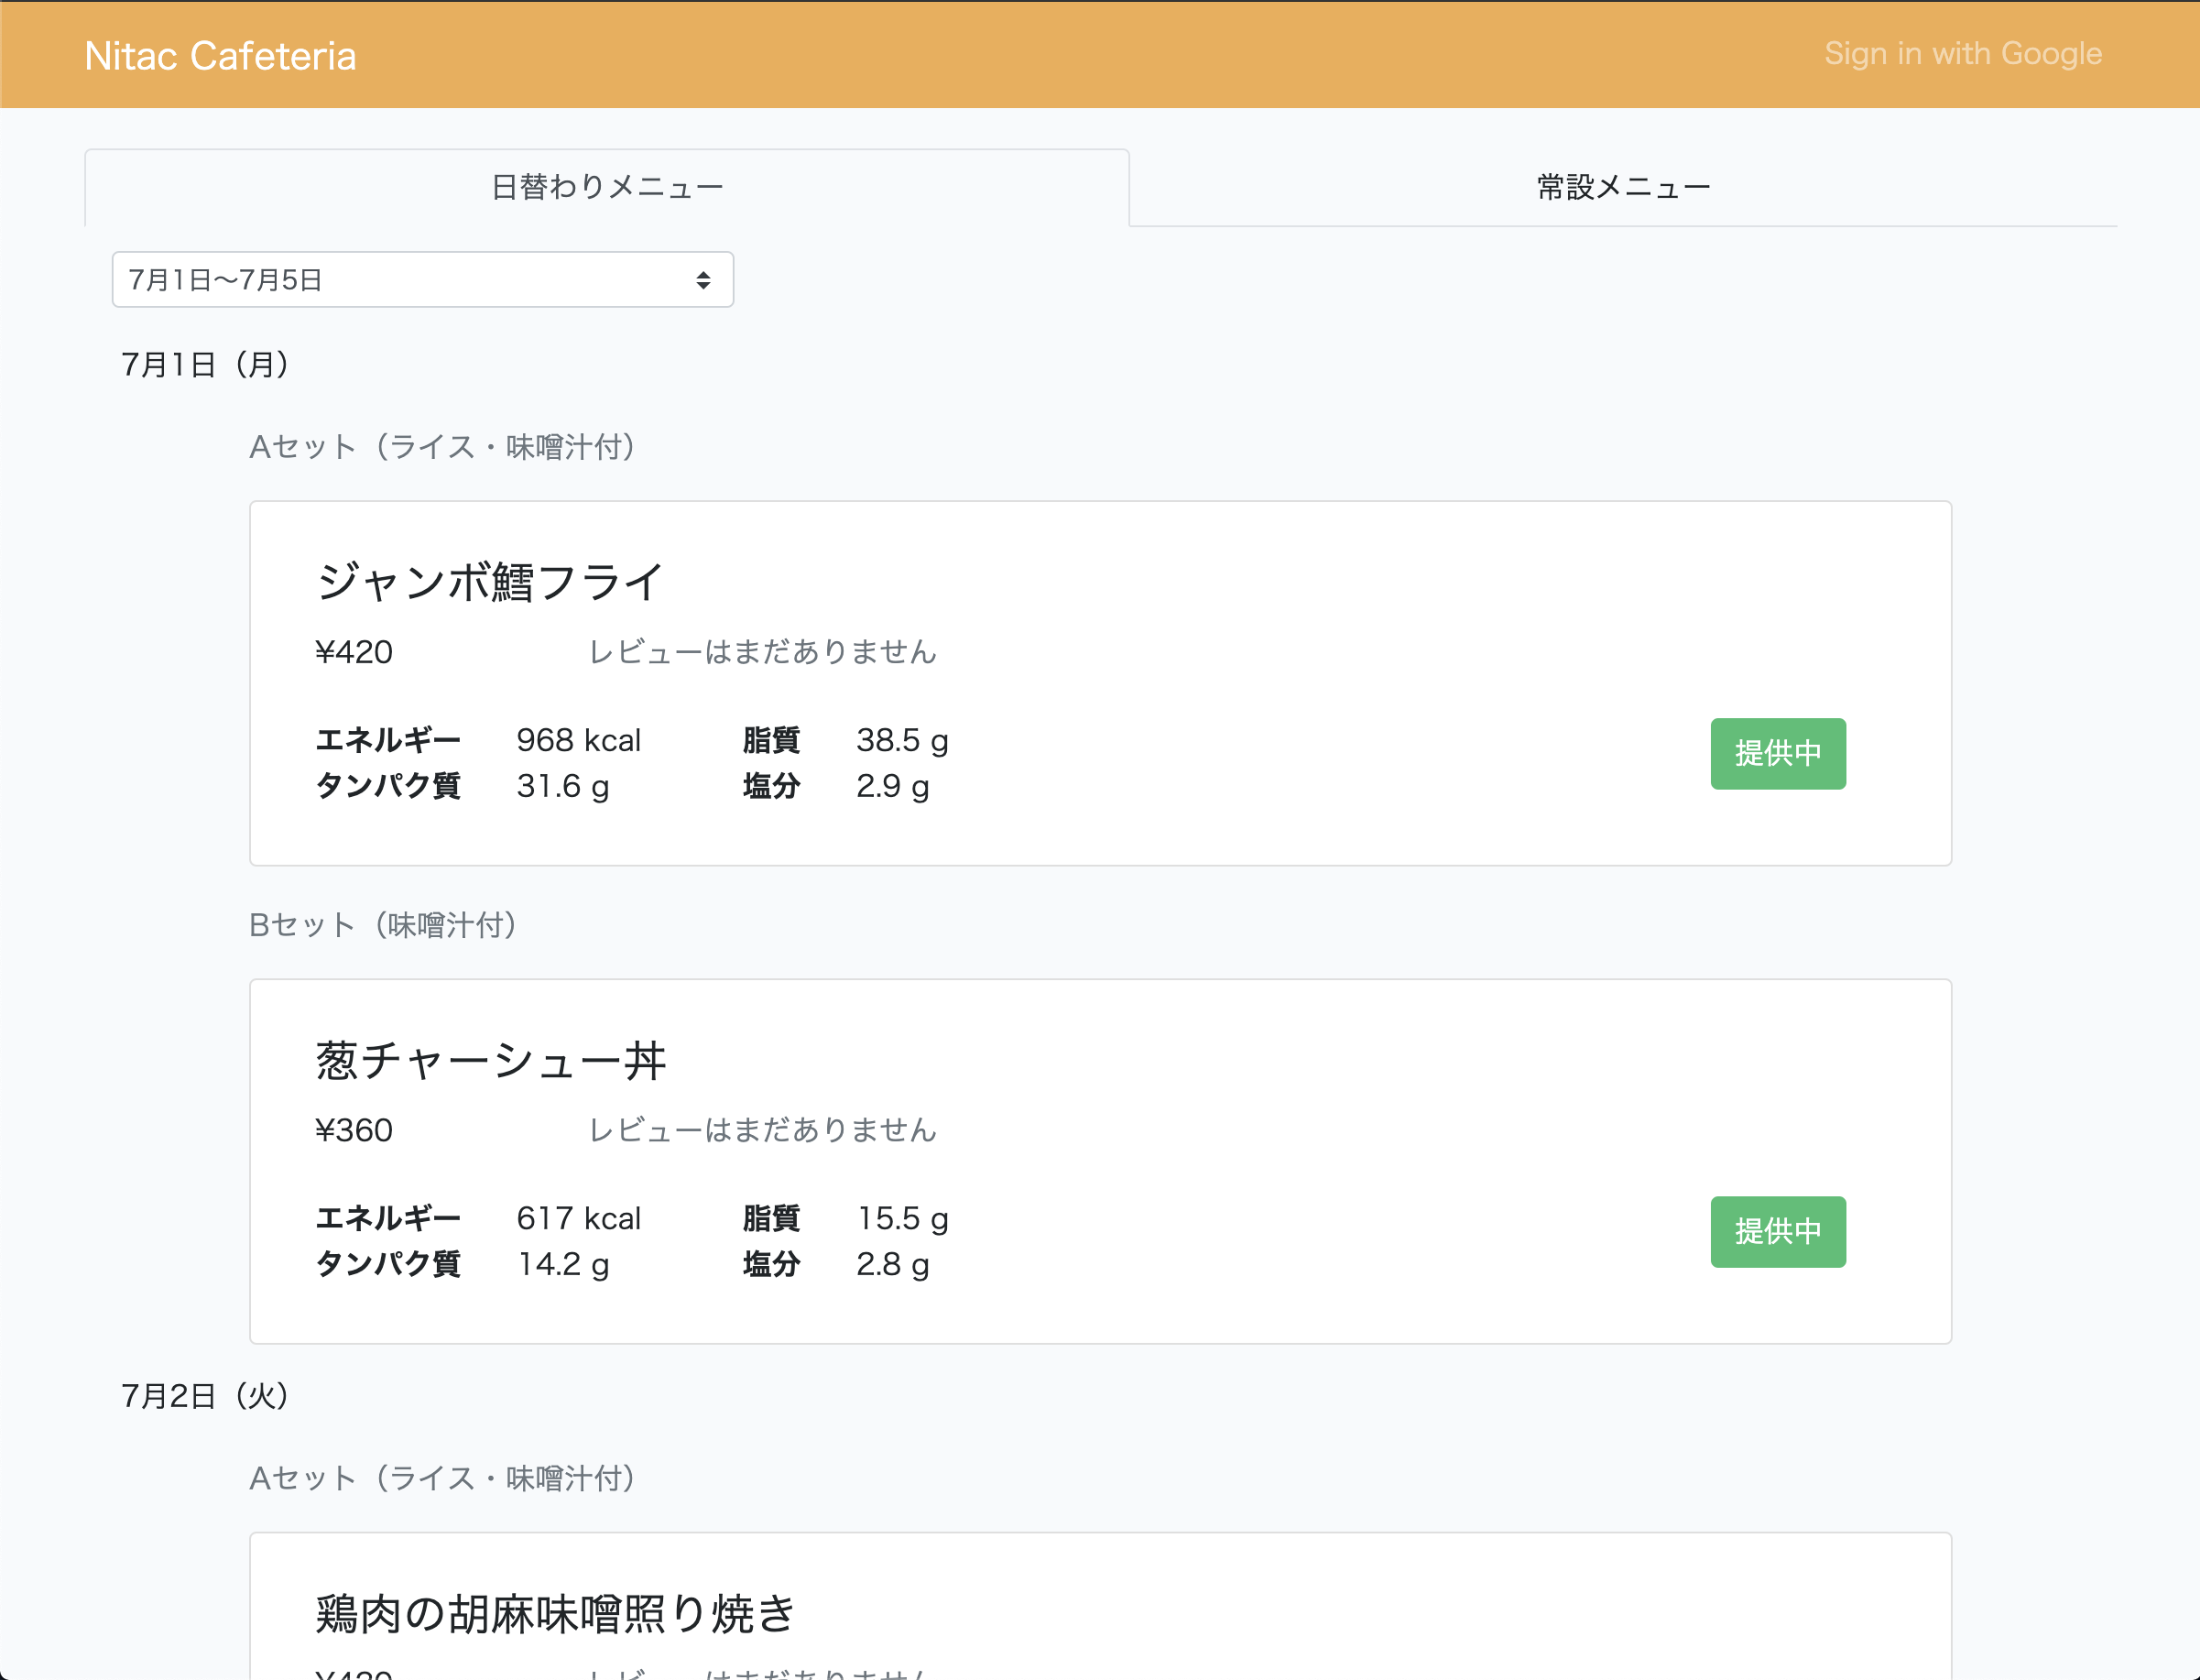
\includegraphics[scale = 0.3]{image/menu.png}
    \end{figure}
    まず最初にメニュー画面が表示されます。
    メニュー画面は日替りメニュー、常設メニューの二つの画面からなり、画面上部にあるタブで切り替えることが出来ます(上図は日替わりメニューの画面)。
    日替りメニュー画面の場合、画面左上にある日付を変更することで表示させたい日付のメニューを表示させることが出来ます。
    \newpage

\subsection{メニューカード}
    \begin{figure}[htbp]
    \centering
        \caption{メニューカード}
        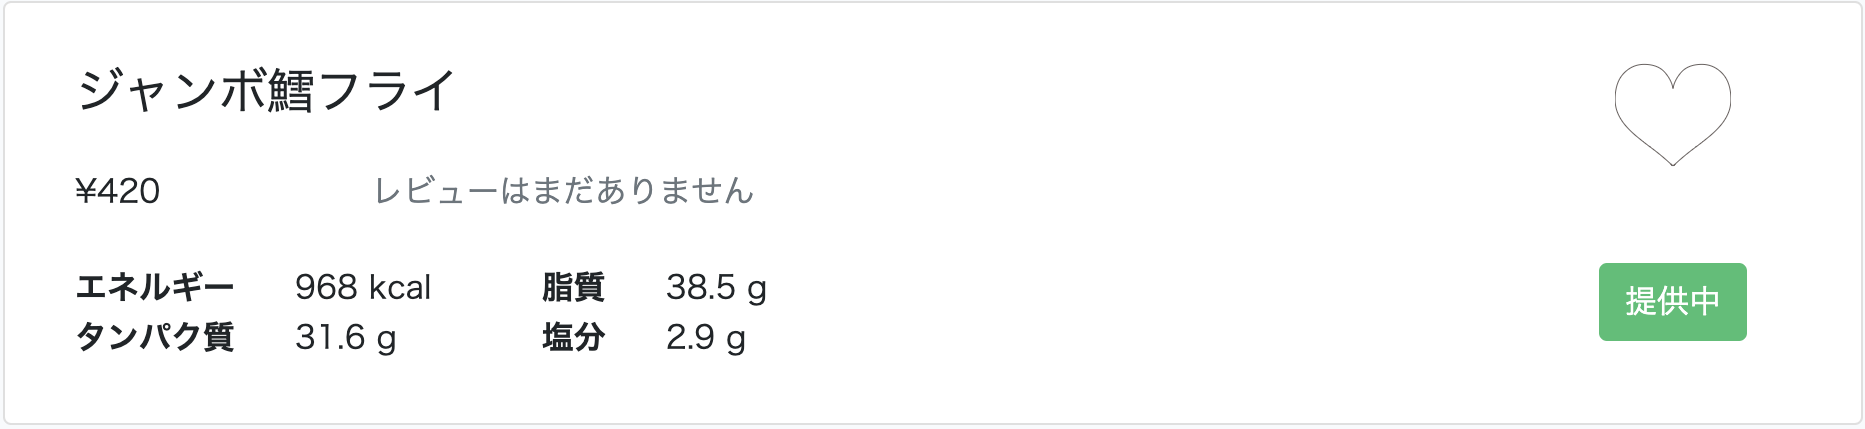
\includegraphics[scale = 0.3]{image/menucard.png}
    \end{figure}

    メニューカードはそれぞれの料理毎に並べられています(図1)。
    カード上の提供中というボタンをクリックすると、売り切れの状態に変化させることが出来ます。
    売り切れの状態なら、売り切れというボタンをクリックすると提供中の状態に変化させる事が出来ます。
    もしあなたがログインしているならば、ハートマークをクリックするとお気に入り登録する事が出来ます。
    またお気に入り登録されたメニューはマイページより確認することが出来ます。

    \begin{figure}[htbp]
    \centering
        \caption{売り切れの状態およびお気に入り登録済みの状態}
        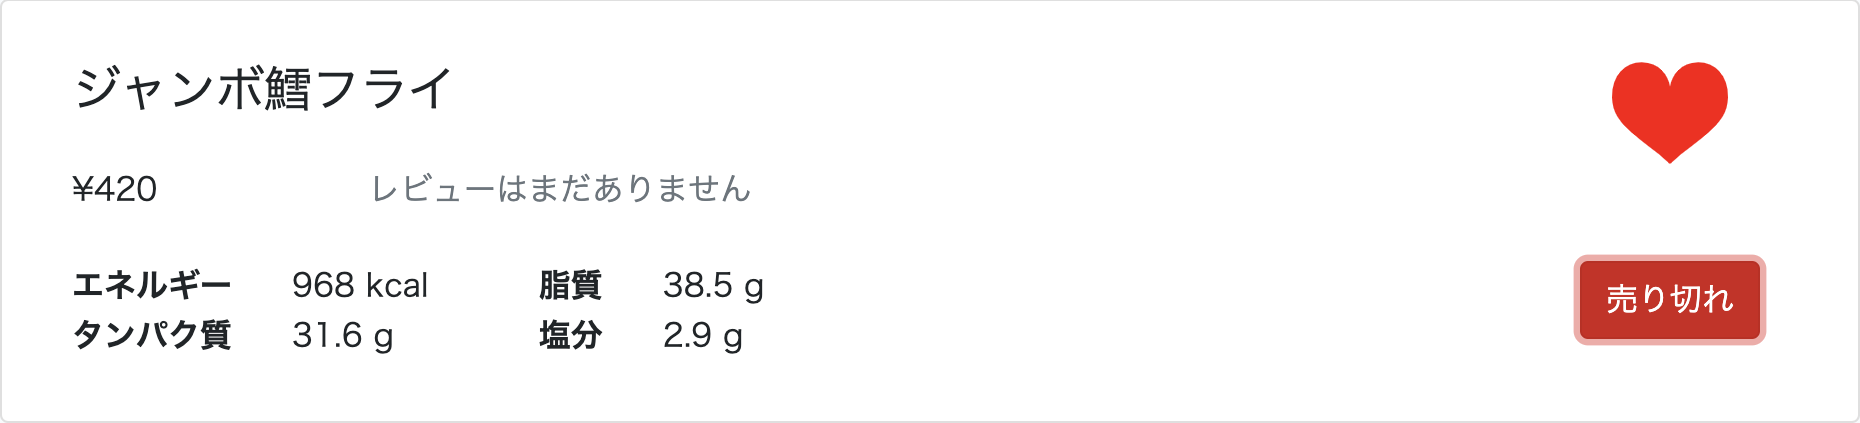
\includegraphics[scale = 0.3]{image/menucard2.png}
    \end{figure}
    メニューカード上のハートマークまたは提供中、売り切れのボタン以外の場所をクリックするとメニュー詳細画面に遷移します。
    \newpage

\section{メニュー詳細画面}
    \begin{figure}[htbp]
    \centering
        \caption{メニュー詳細画面}
        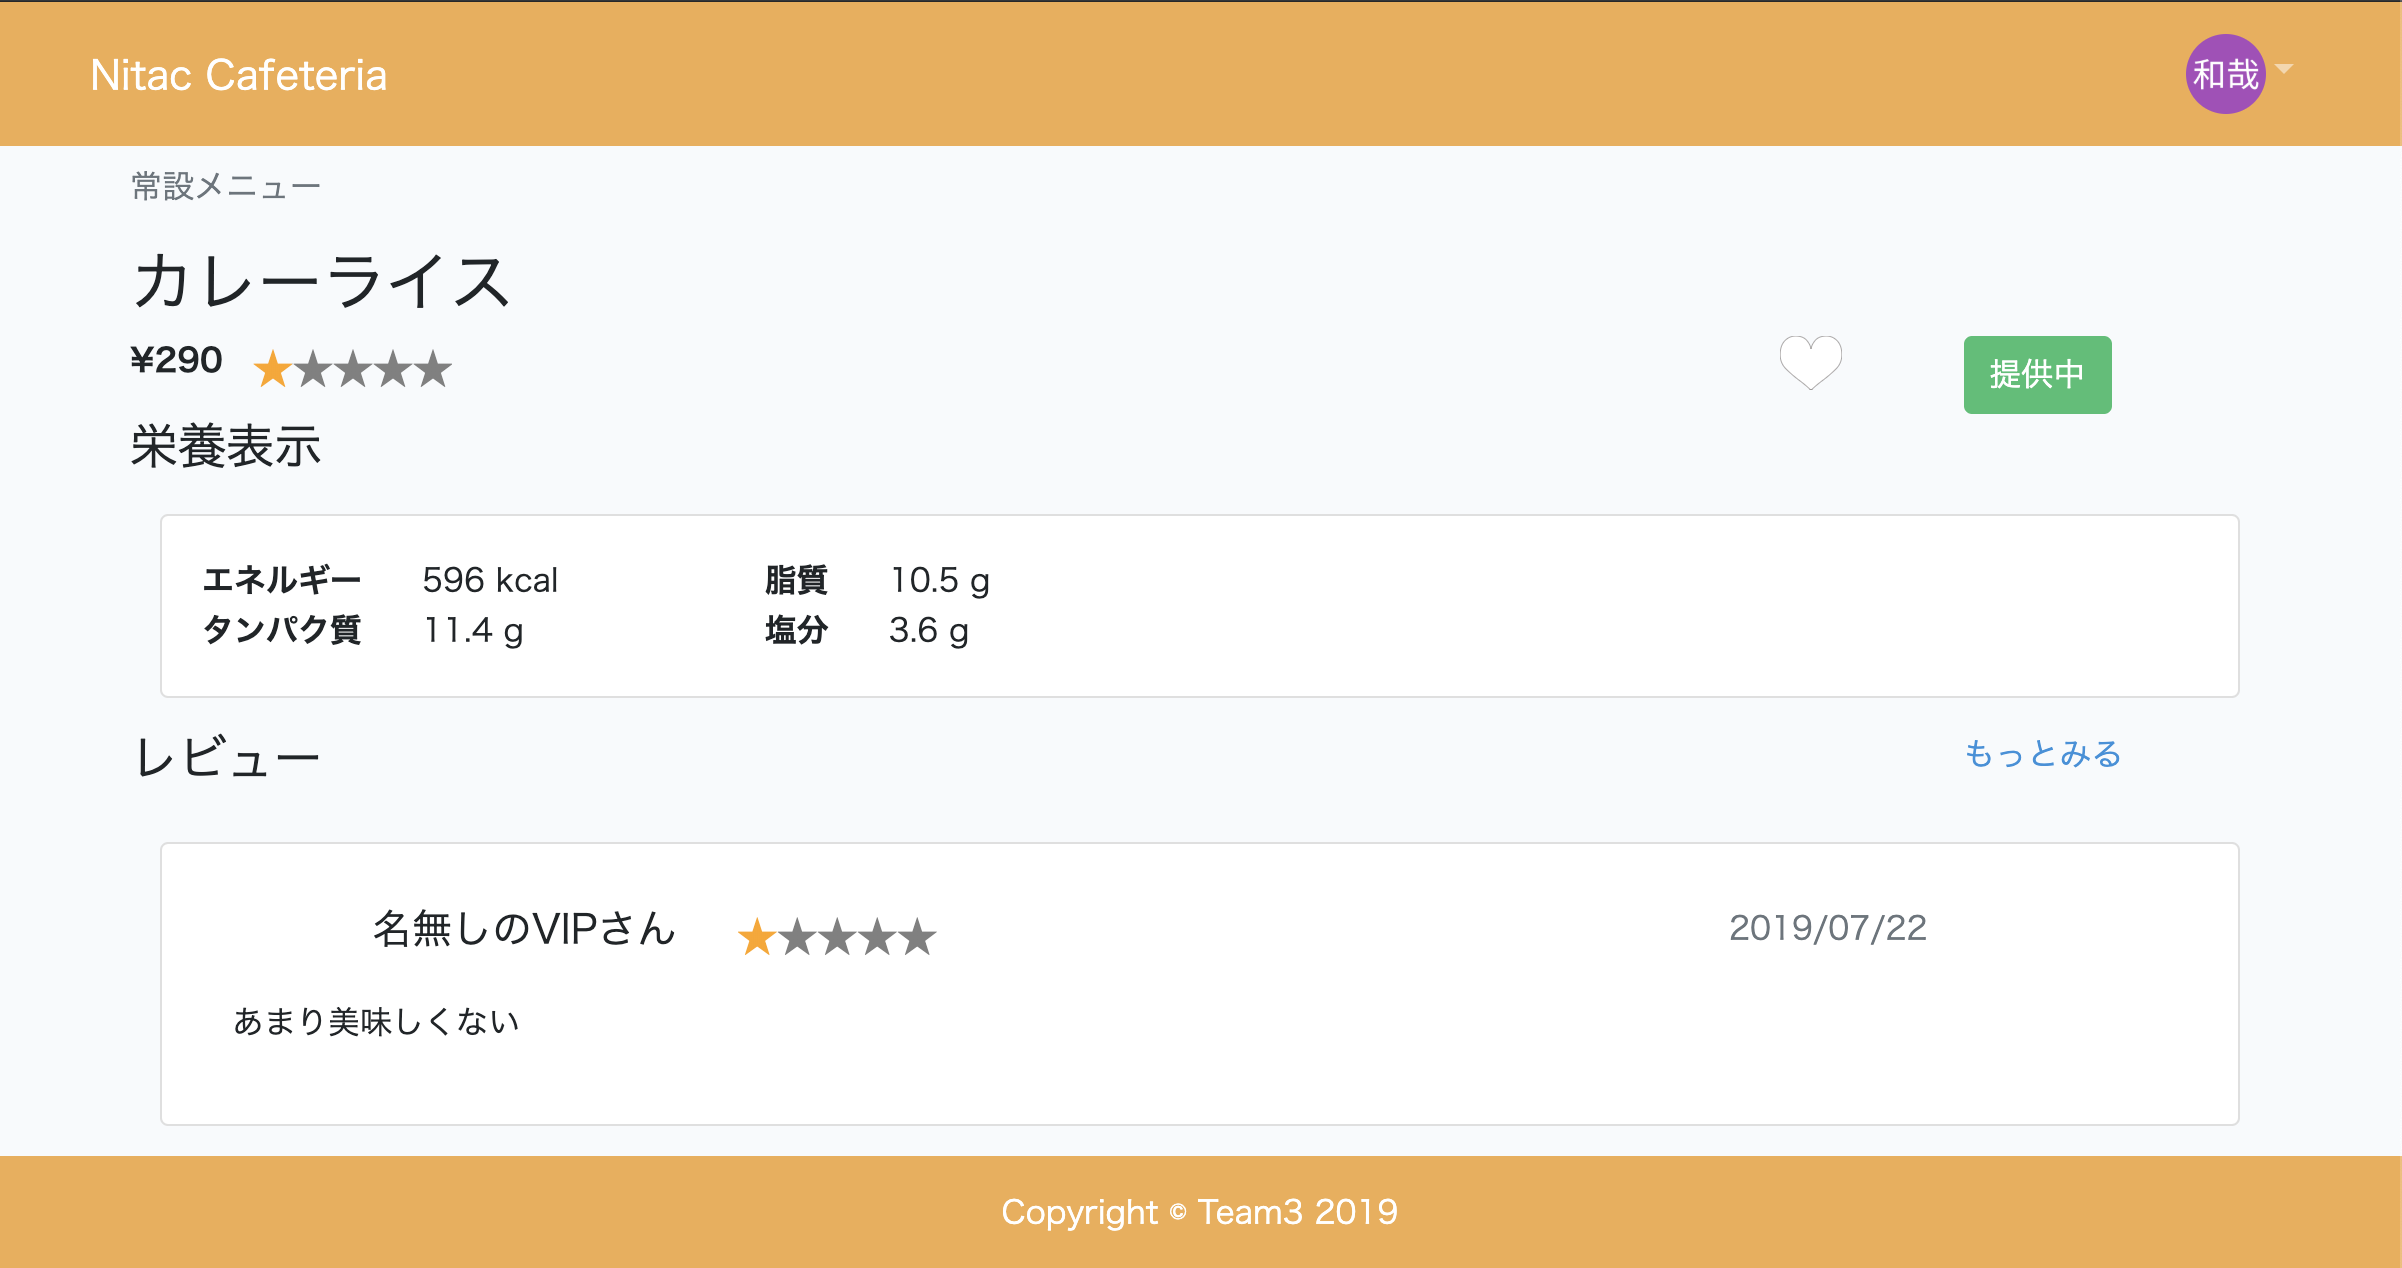
\includegraphics[scale = 0.3]{image/detail.png}
    \end{figure}
    メニュー詳細画面では他のユーザーが投稿したメニューの画像及びレビュー等を閲覧することが出来ます。
    ここでも提供中または売り切れのボタンをクレックする事でその状態を変化させることが出来ます。
    画面右中部にある「もっと見る」をクリックすることによって、レビュー一覧画面に遷移する事が出来ます。

\subsection{レビュー一覧画面}
    \begin{figure}[htbp]
    \centering
        \caption{レビュー一覧画面}
        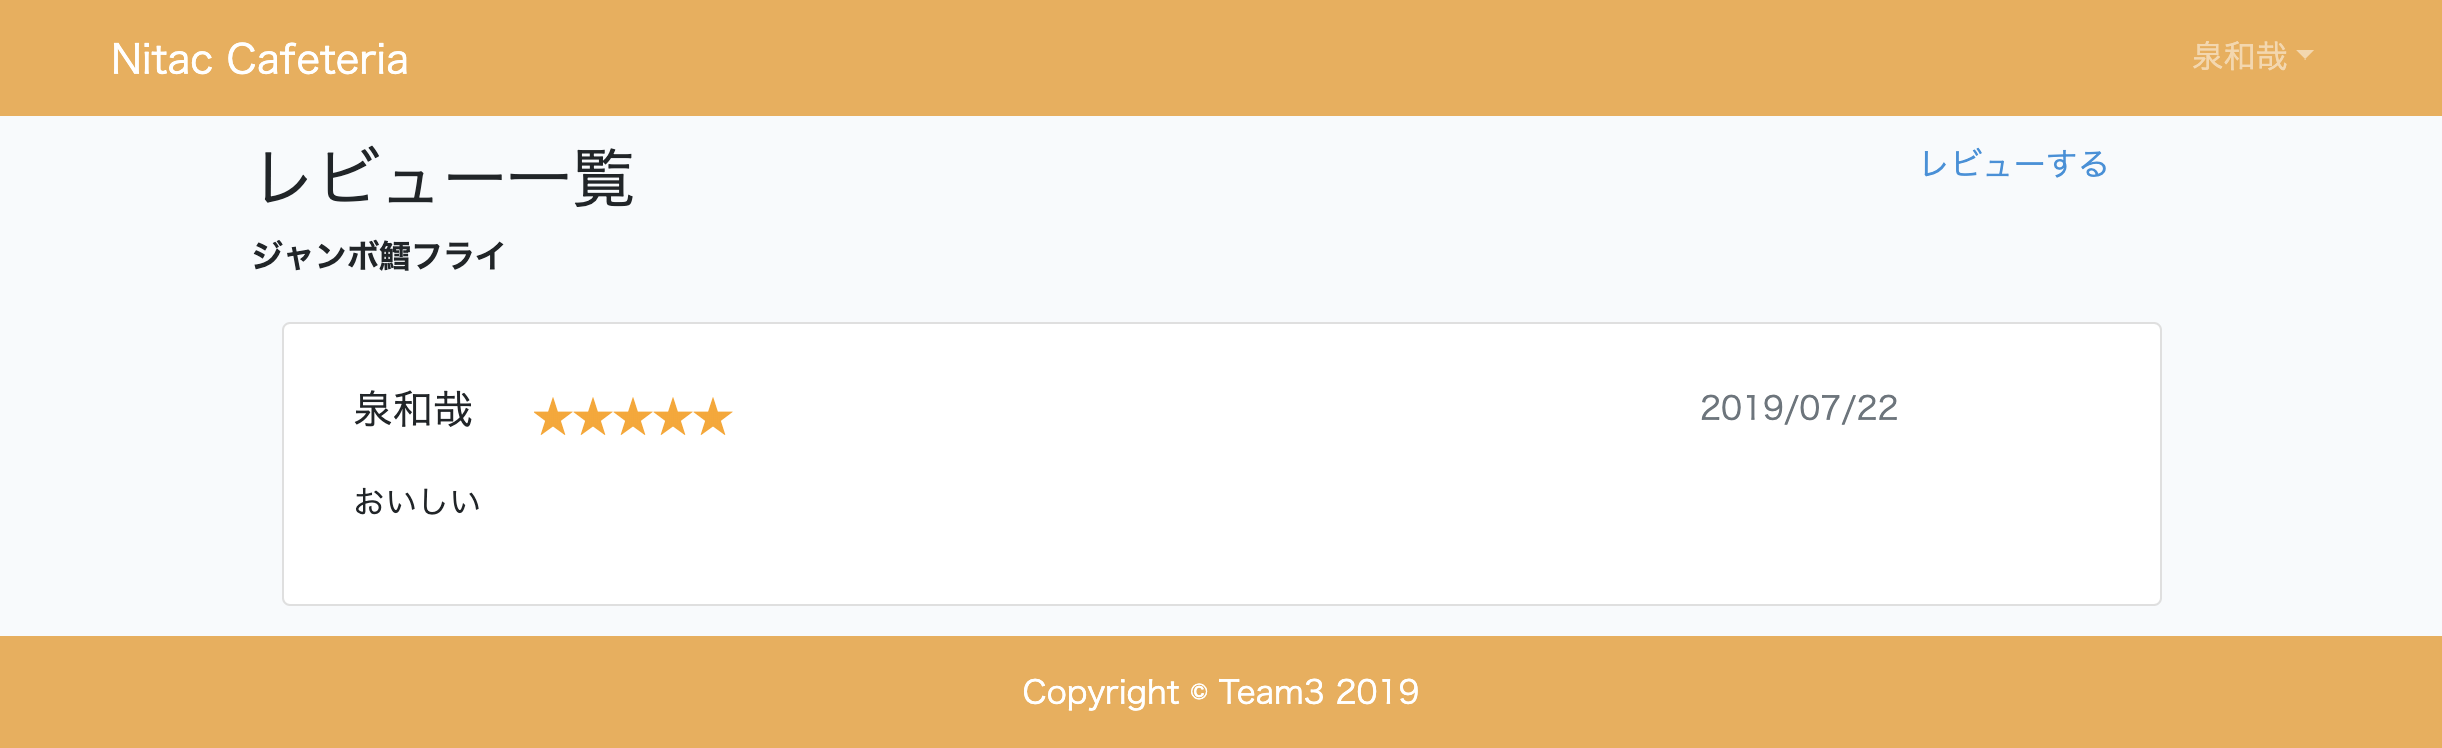
\includegraphics[scale = 0.3]{image/review.png}
    \end{figure}
    レビュー一覧画面では、全てのユーザーのレビューを閲覧する事が出来ます。
    また、画面右上部にある「レビューする」をクリックするとレビュー画面に遷移する事が出来ます。
    但し、ログインした状態でなければ「レビューをする」が表示されずレビューをする事は出来ません。
    \newpage

\subsection{レビュー画面}
    \begin{figure}[htbp]
    \centering
        \caption{レビュー画面}
        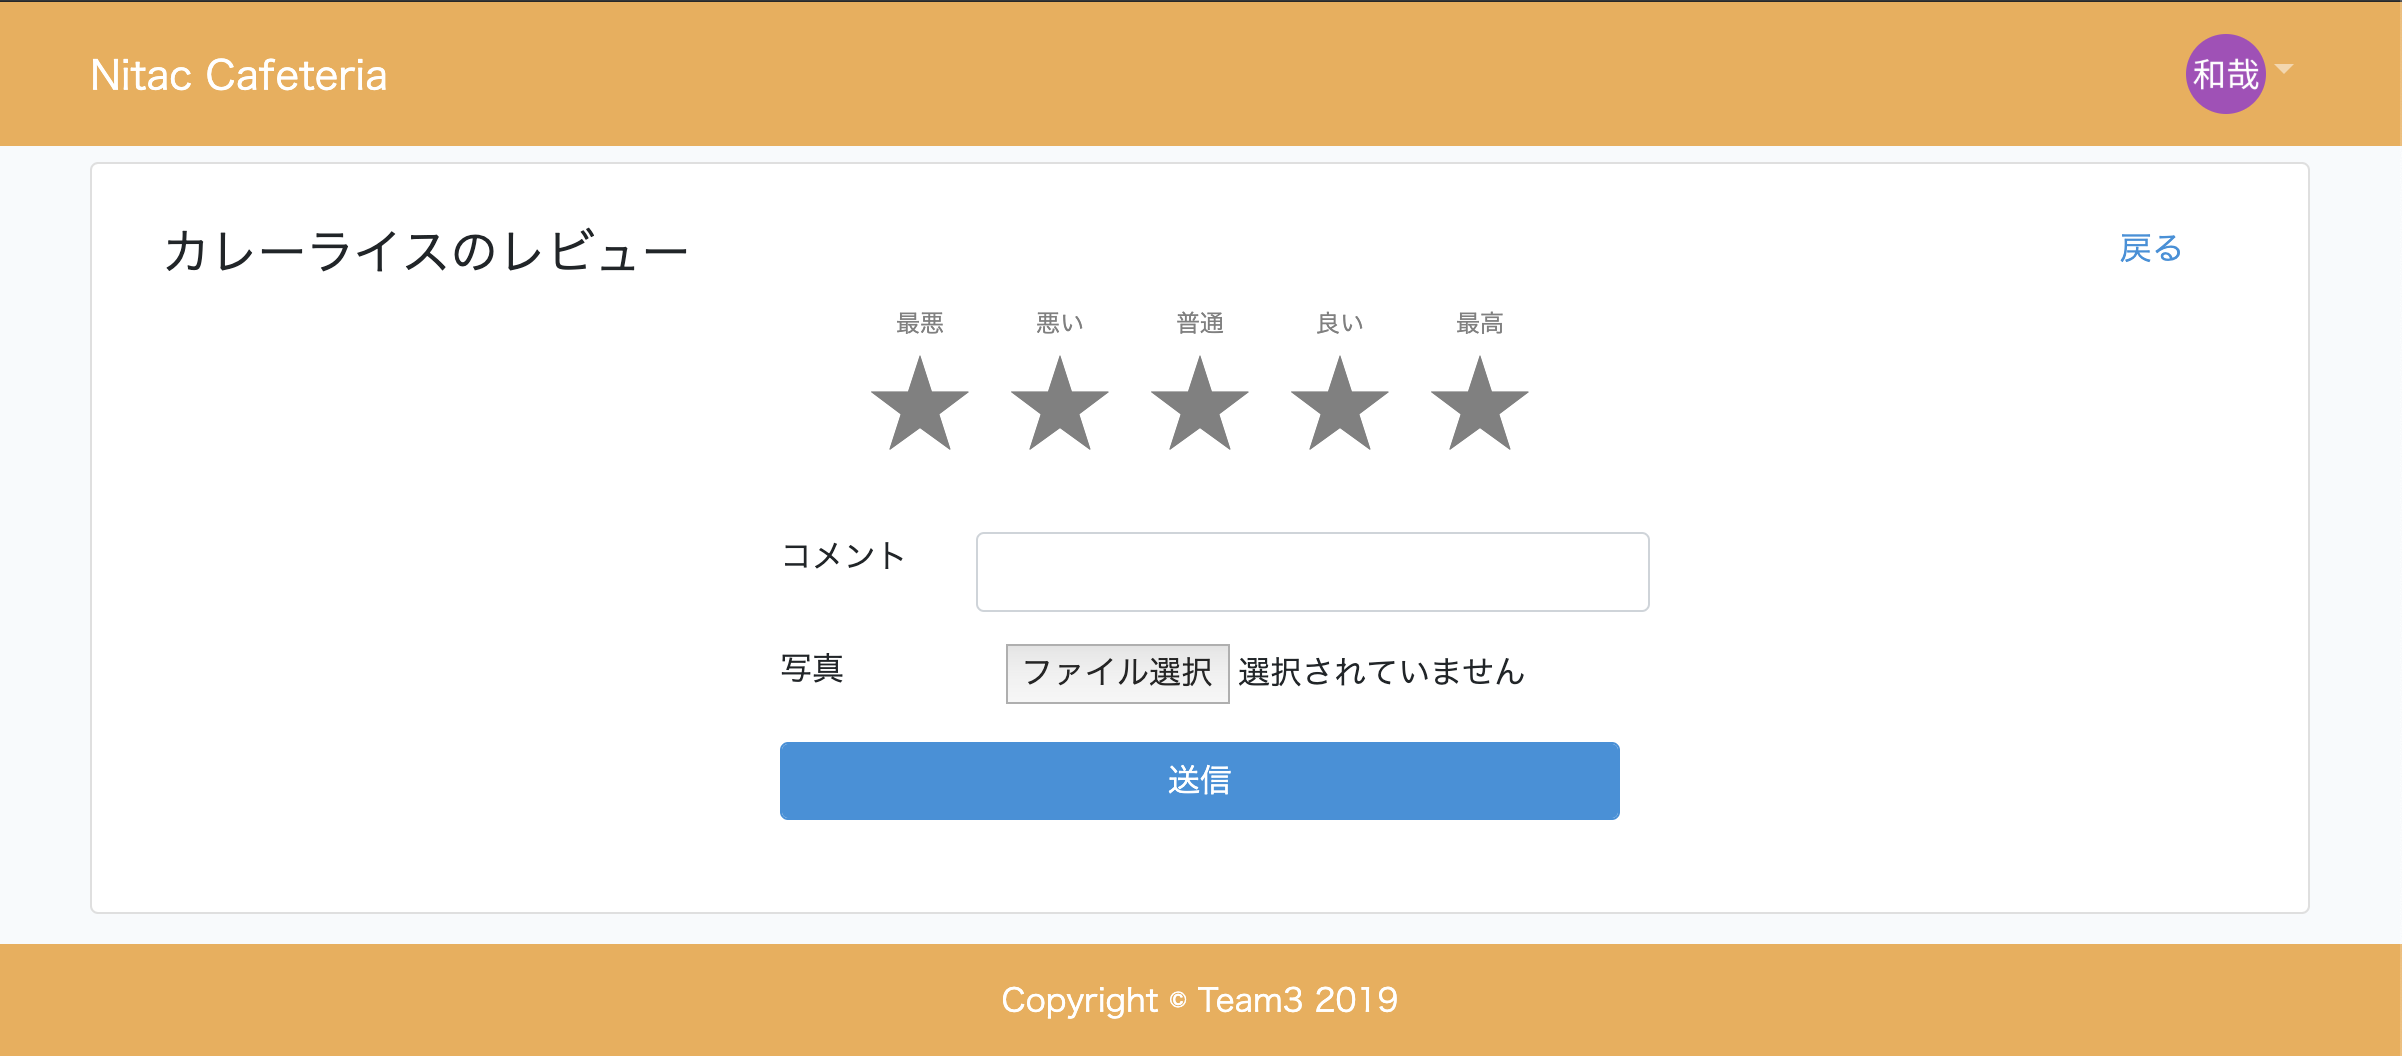
\includegraphics[scale = 0.3]{image/review2.png}
    \end{figure}
    レビュー画面ではメニューを五段階評価(星の数)で評価し、コメント及び写真を投稿する事が出来ます。
    星の数やコメントなどの設定が完了しましたら、送信ボタンをクリックする事でレビューを投稿する事が出来ます。
    投稿された写真はメニュー詳細画面(図4)上部の写真の位置に反映されます。
    投稿されたレビューは、そのメニューのレビュー一覧画面(図5)、マイページから確認する事が出来ます。

\section{ログイン}
    画面右上(図1)のアイコンをクリックして、表示されたドロップダウンの中にある「Sign in with Google」をクリックすると、ログイン画面に遷移します。
    ログインにはGoogleアカウントが必要なので、お持ちでない方はアカウントを作成して頂く必要があります。
    \begin{figure}[htbp]
    \centering
        \caption{ログイン画面}
        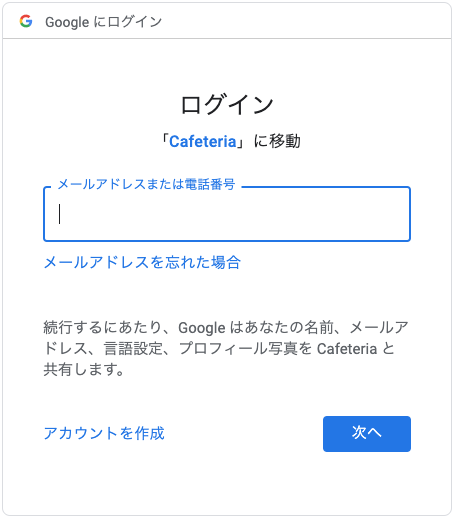
\includegraphics[scale = 0.3]{image/login.png}
    \end{figure}

\section{ログアウト}
    画面右上(図1)のアイコンをクリックして、表示されたドロップダウンの中にある「ログアウト」をクリックすると、ログアウトが完了します。

\section{マイページ}
    画面右上(図1)のアイコンをクリックして、表示されたドロップダウンの中にある「マイページ」をクリックすると、マイページに遷移します。但し、この操作にはログインが必要です。
    \begin{figure}[htbp]
    \centering
        \caption{マイページ仮画面}
        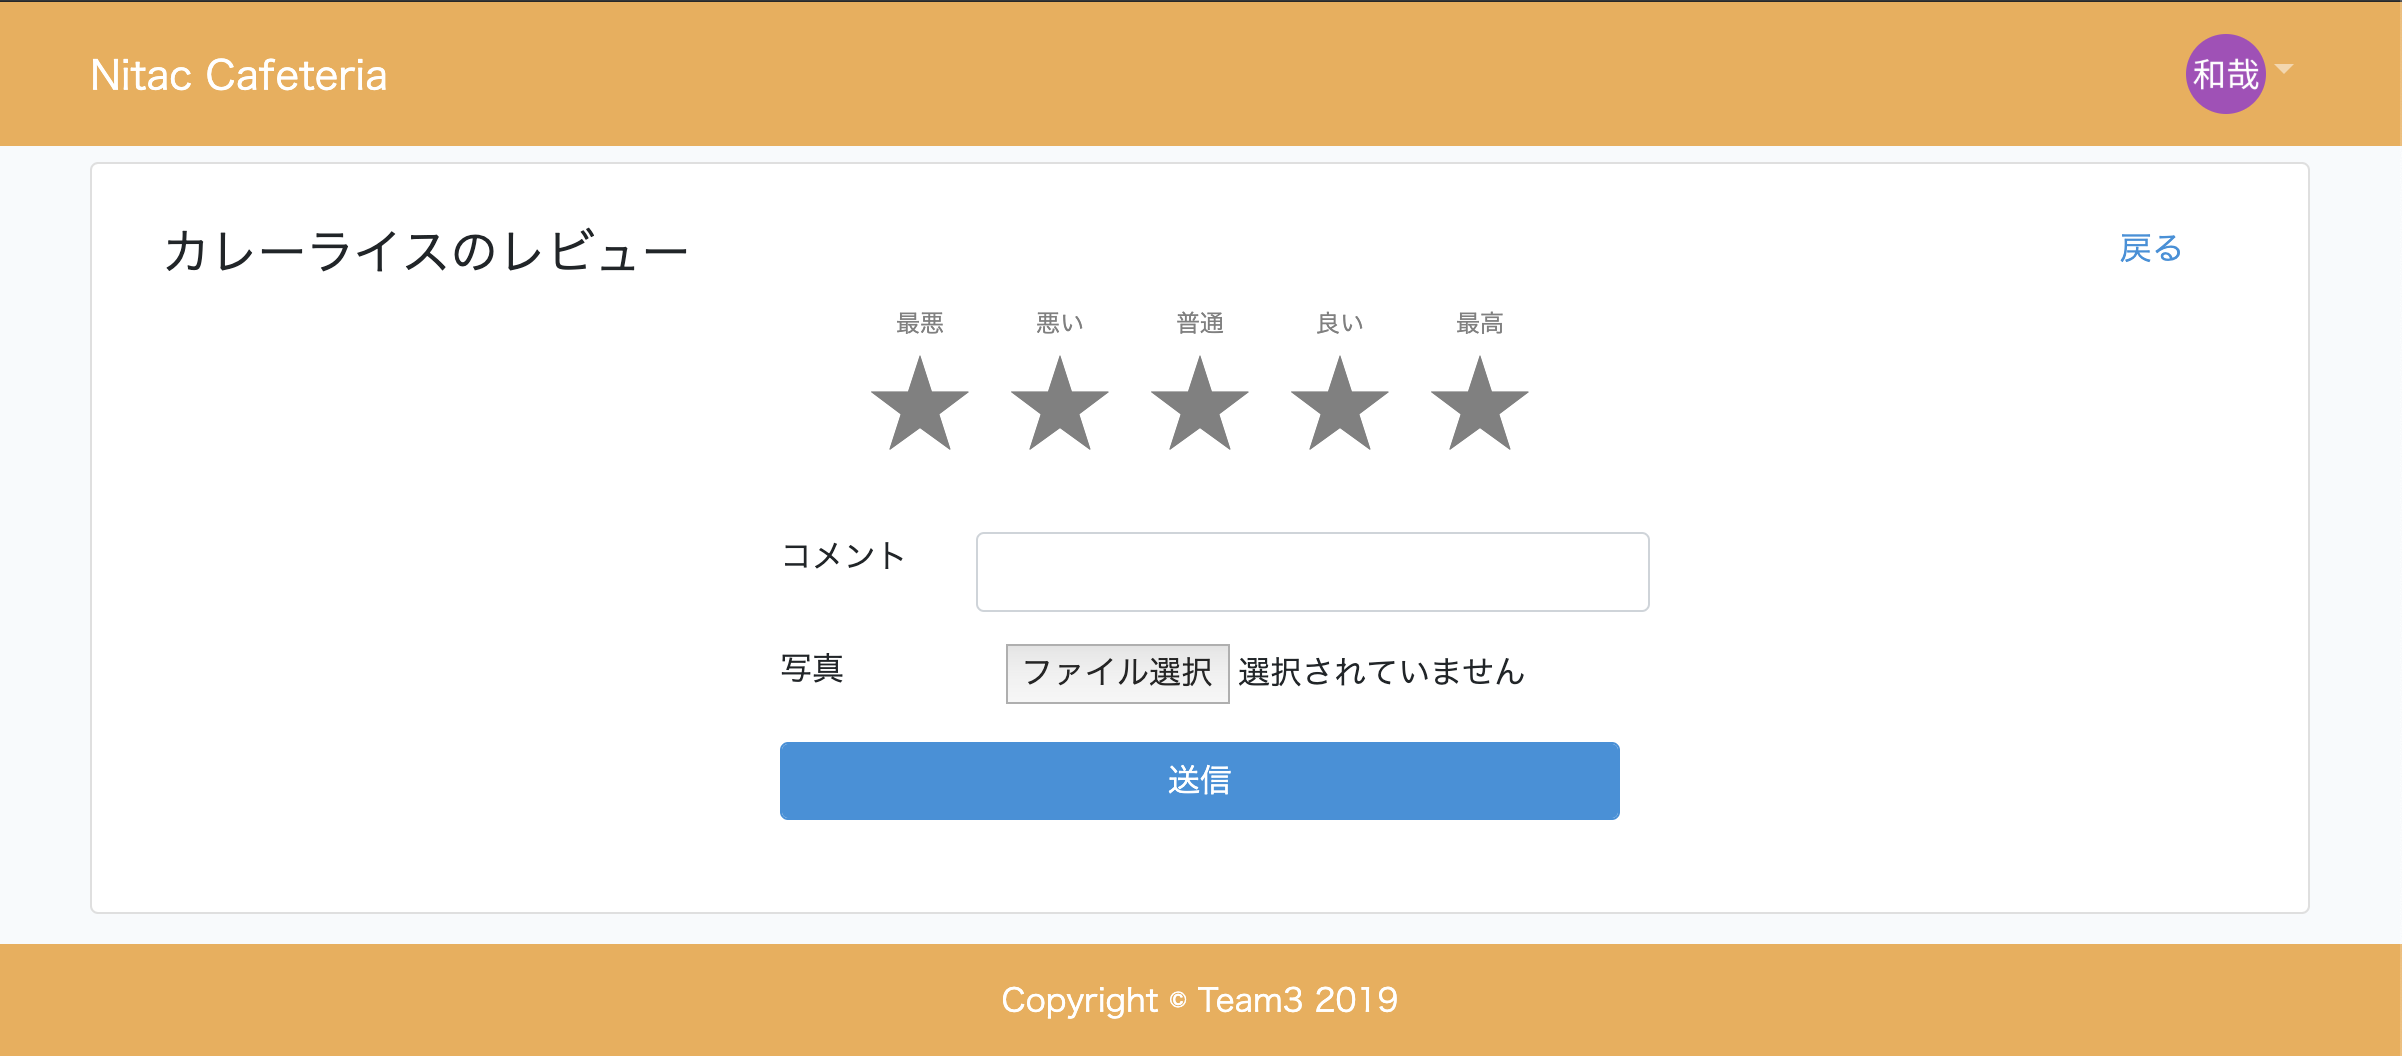
\includegraphics[scale = 0.3]{image/review2.png}
    \end{figure}
    \newpage

    \subsection{マイページ・レビュー一覧画面}
        マイページから「レビュー」をクリックすると今までに投稿したレビューを確認する事が出来ます(図9)。
        \begin{figure}[htbp]
        \centering
            \caption{マイページ・レビュー一覧画面}
            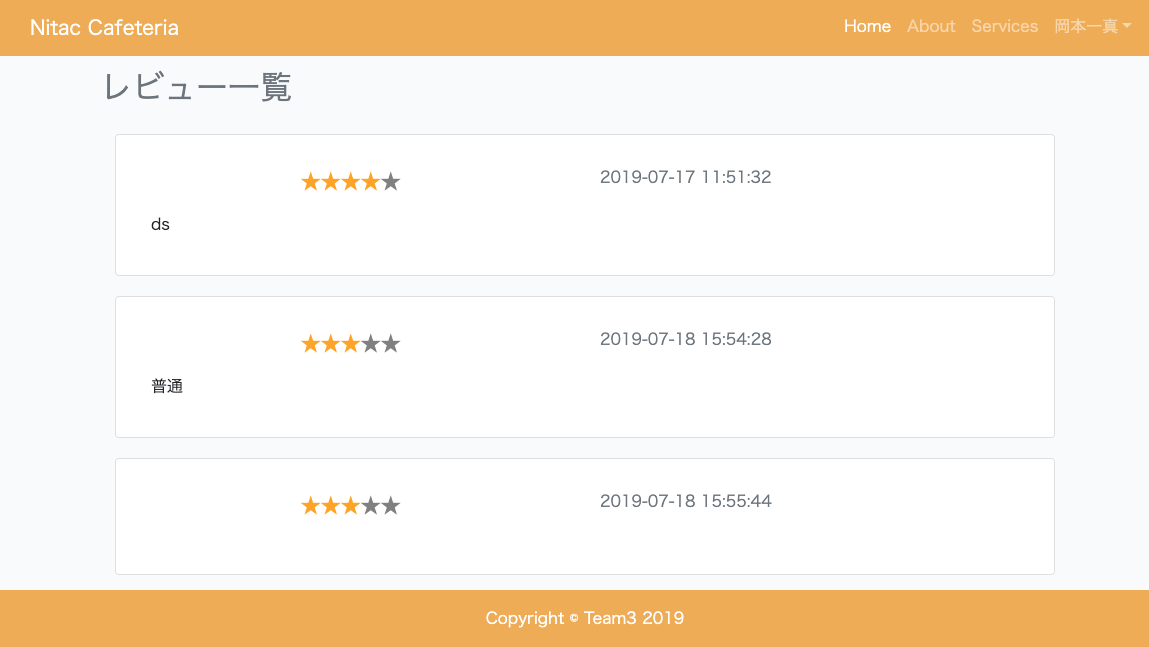
\includegraphics[scale = 0.3]{image/myreview.png}
        \end{figure}

    \subsection{マイページ・お気に入り画面}
        マイページから「お気に入り」をクリックすると今までにお気に入り登録したメニューを確認することが出来ます。
        \begin{figure}[htbp]
        \centering
            \caption{マイページ・お気に入り画面}
            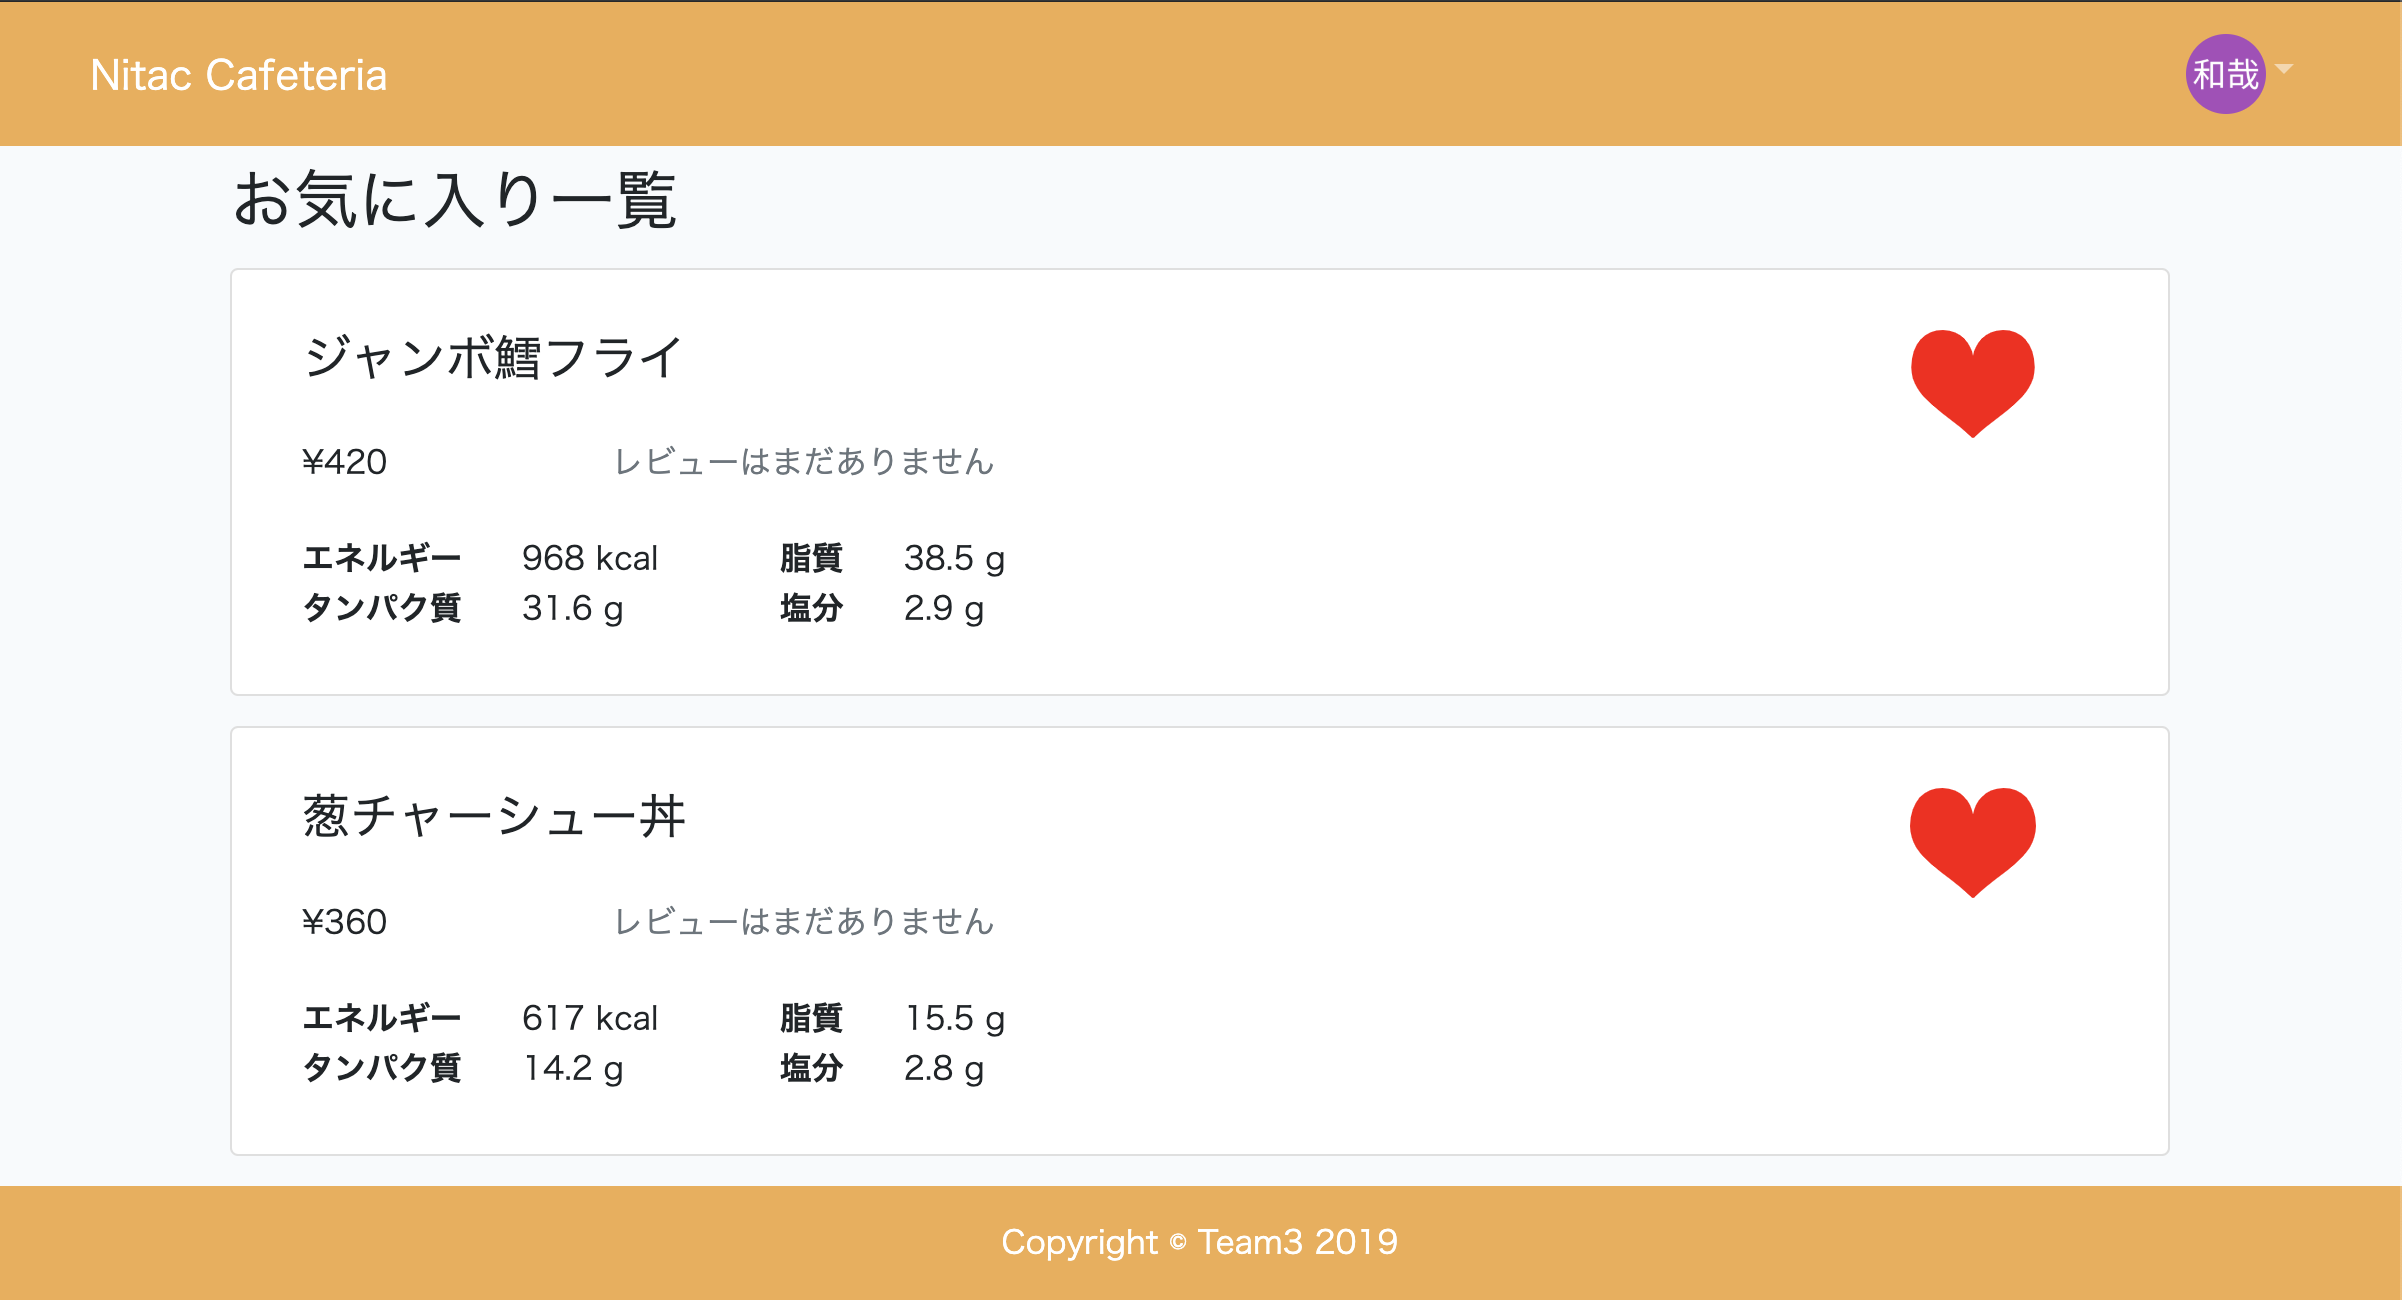
\includegraphics[scale = 0.3]{image/myfavorite.png}
        \end{figure}
        \newpage

\section{管理者用画面}
    \subsection{メニュー登録画面}
        \begin{figure}[htbp]
        \centering
            \caption{メニュー登録画面(かり)}
            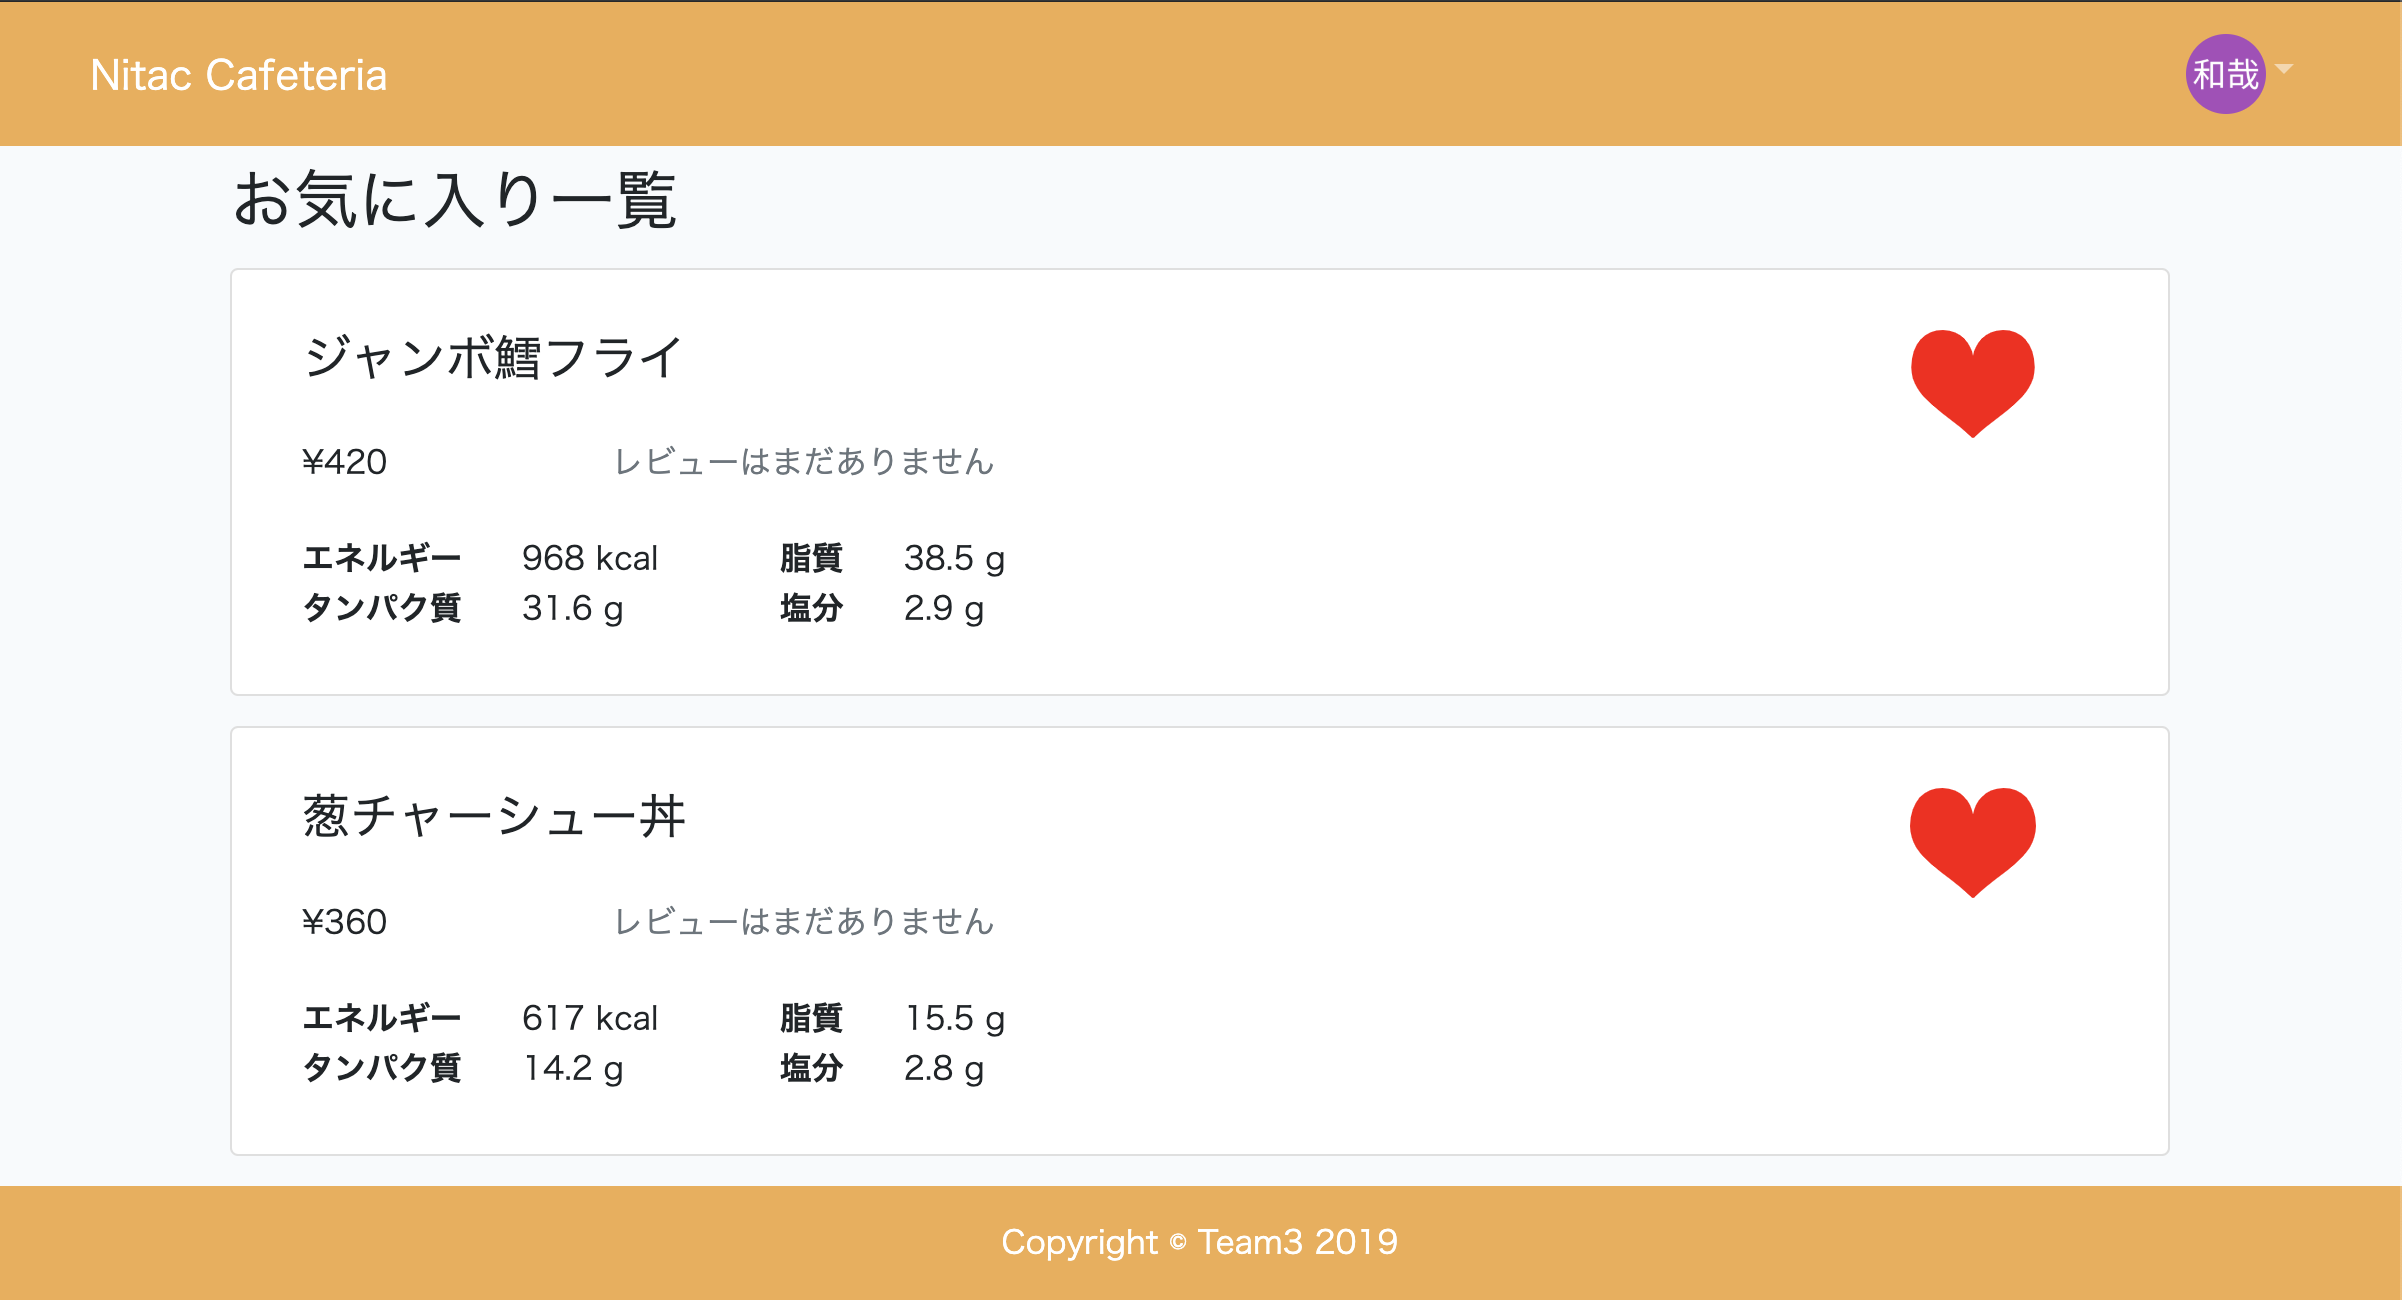
\includegraphics[scale = 0.3]{image/myfavorite.png}
        \end{figure}
        この画面では、メニューの登録を行う事が出来ます。
        各項目を入力した後に、Submitをクリックすると登録が完了します。

    \subsection{メニューセット画面}
        \begin{figure}[htbp]
        \centering
            \caption{メニューセット画面(かり)}
            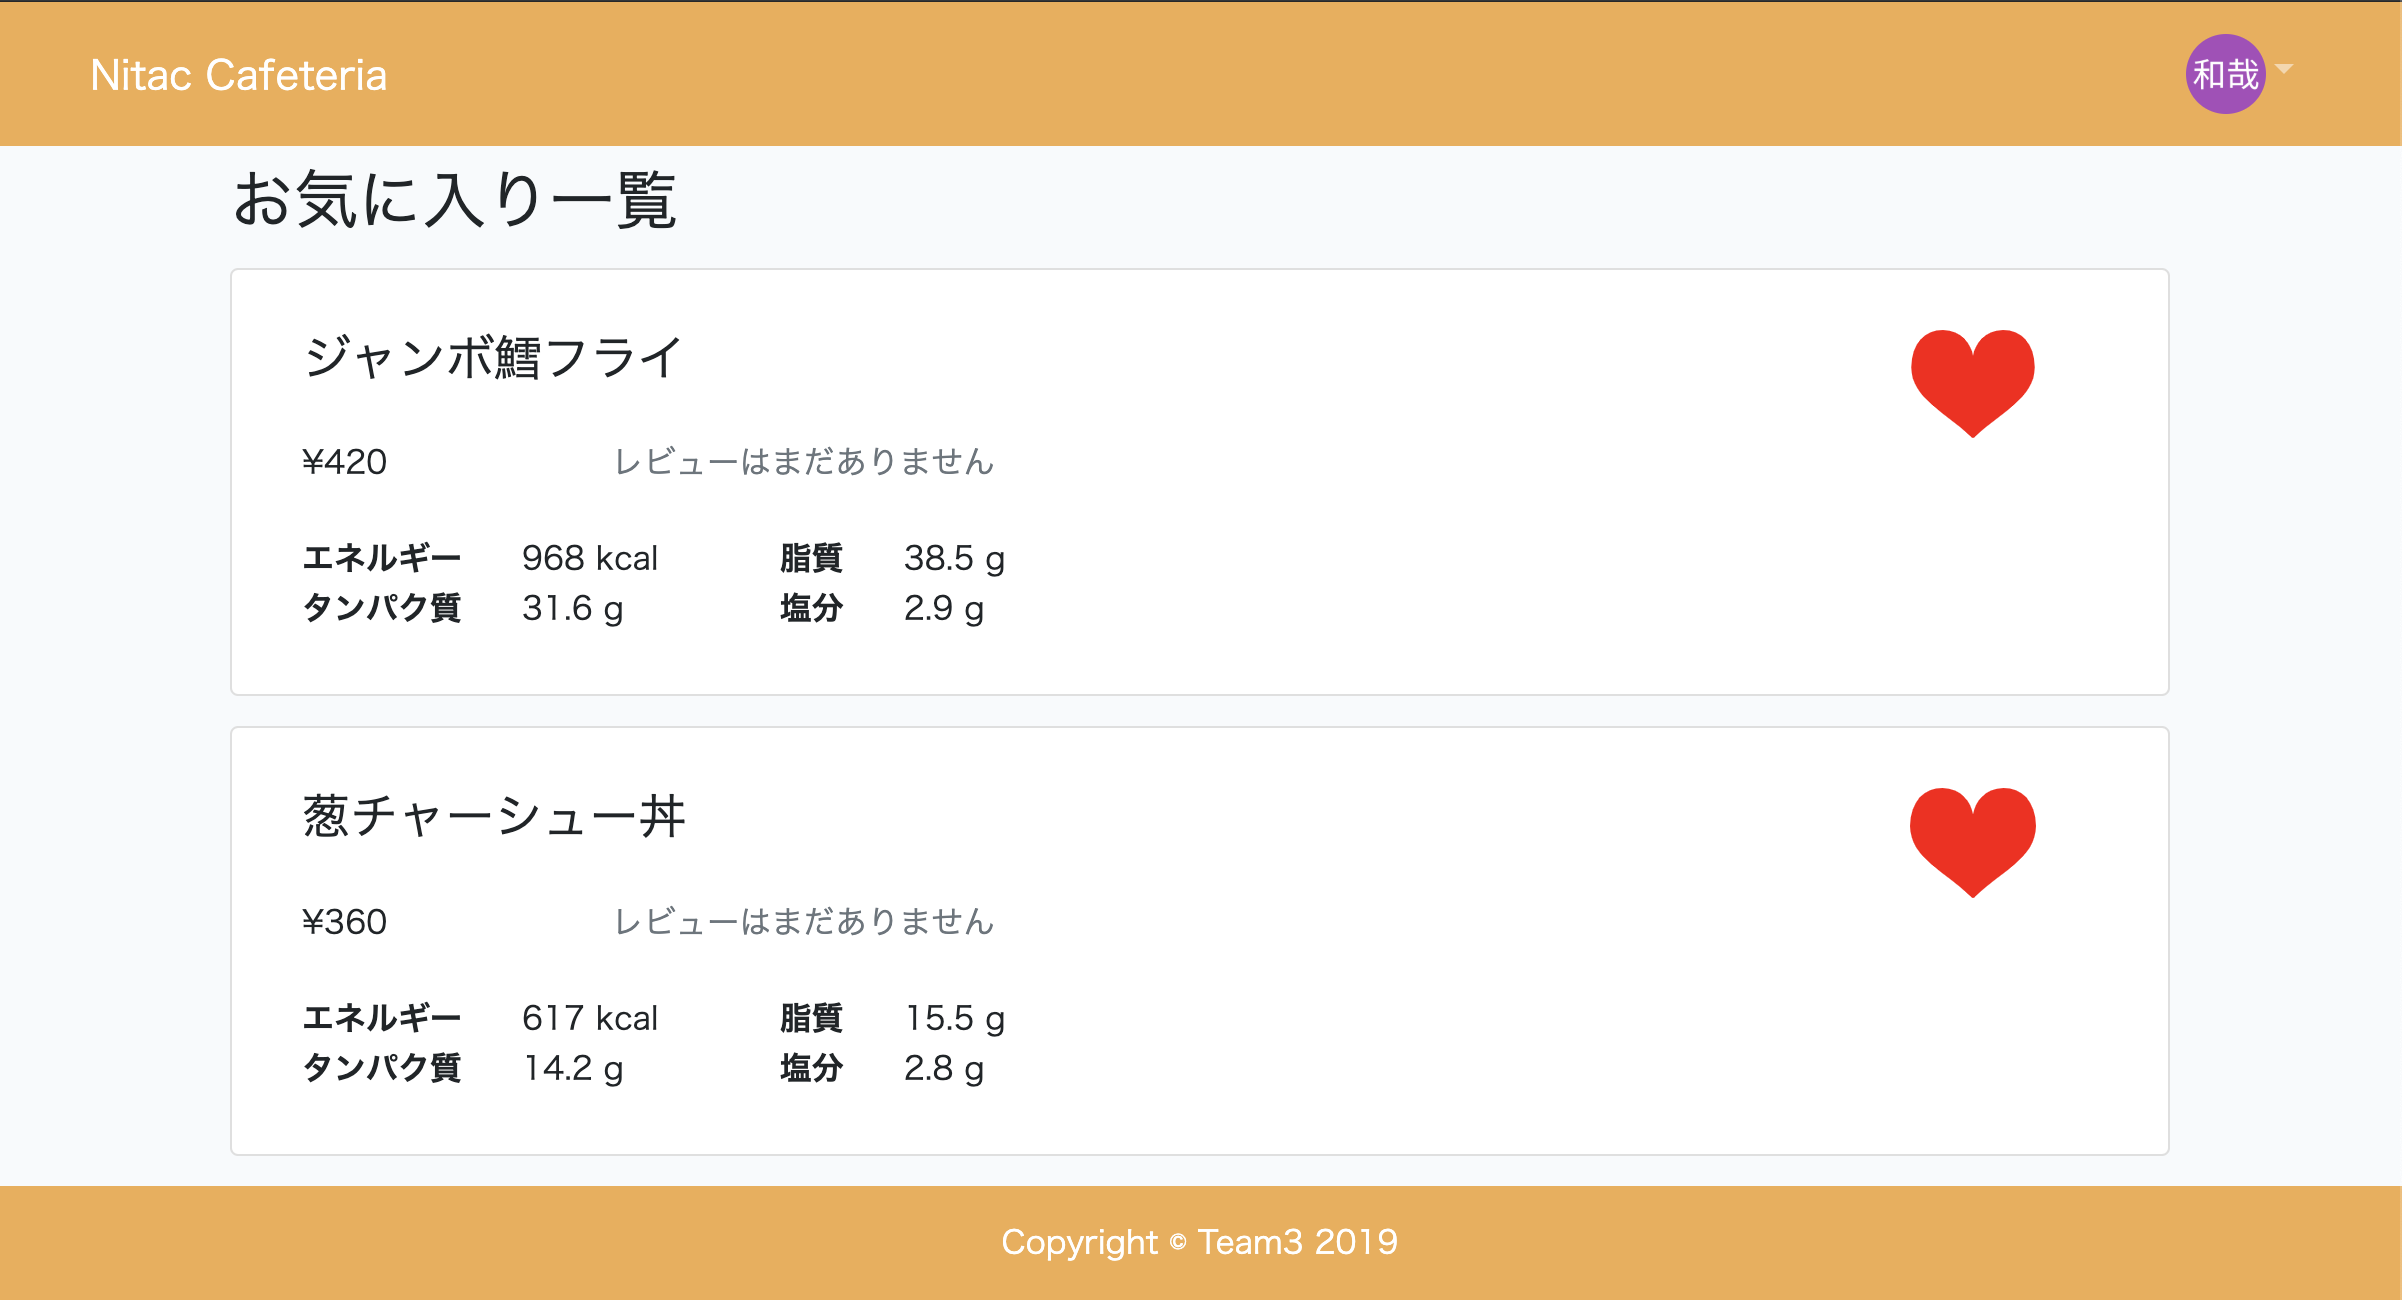
\includegraphics[scale = 0.3]{image/myfavorite.png}
        \end{figure}
        この画面では、メニューのセットを行うことが出来ます。

\end{document}
